\documentclass{article}
\usepackage[utf8]{inputenc}

\usepackage{graphicx}
\usepackage[margin=1.25in]{geometry}
\usepackage{float}

\title{CS347 Coursework: Raft Consensus Algorithm}
\author{Luke Mills \and Ben Metzger \and Radu Cobianu \and Josh Featherstone \and Michael Lim \and Alexander Price}

\begin{document}

\maketitle

\section{Abstract}

This is an example abstract.

\section{Introduction}

\section{Research}

\section{Requirements Analysis}

    \begin{figure}[H]
        \centering
        \fbox{
            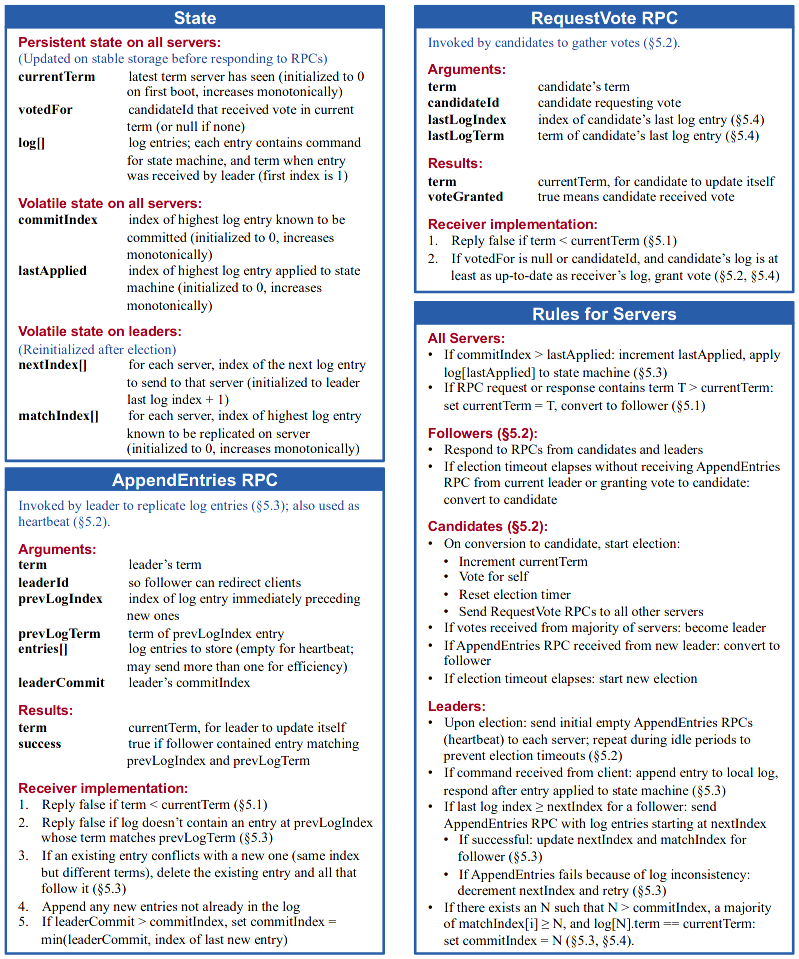
\includegraphics[width=\textwidth]{./resources/condensedsummary.png}
        }
        \caption{`A condensed summary of the Raft consensus algorithm' [REFERENCE] }
        \label{fig:condensedsummary}
    \end{figure}
    
    In addition to the requirements specified in the condensed summary, the paper specifies behaviour for membership changes and log compaction.
    \subsection{Cluster Membership Changes}
    The requirements below specify behaviour in the case where the set of participating servers changes. Here `cluster configuration' refers to a set of servers.
    
    \noindent \begin{tabular}{|p{0.1\textwidth}|p{0.85\textwidth}|}
        \hline
        \multicolumn{2}{|c|}{General Requirements}  \\ \hline
        M.1 & Cluster configurations are stored and communicated using special entries in the replicated log. \\ \hline
        M.2 & A server must always use the latest configuration in its log for any decisions, regardless of whether it has been committed or not. \\ \hline
        M.3 & When moving from an old configuration to a new configuration, the cluster must first move to a transitional state (`joint consensus'). The joint consensus configuration is the combination of the old configuration and the new configuration, i.e. the union of the two sets of servers.\\ \hline
        M.4 & Before a configuration change, new servers must join the cluster as non-voting members. Entries in the log are replicated to these servers, but they are not considered for majorities. \\ \hline
    \end{tabular}
    
    \hspace{2em}
    
    \noindent \begin{tabular}{|p{0.1\textwidth}|p{0.85\textwidth}|}
        \hline
        \multicolumn{2}{|c|}{Leader Requirements}  \\ \hline
        M.OL.1 & When the old configuration leader receives a request to change the configuration ($C_{old}\rightarrow C_{new}$), it must store the configuration for joint consensus ($C_{old}C_{new}$) as a log entry and replicate the entry to the servers in this configuration, determining when this entry has been committed using the joint consensus configuration. \\ \hline
        M.OL.2 & After successfully committing the joint consensus configuration, the leader must store the new configuration ($C_{new}$) as a log entry and replicate the entry to the cluster (all servers in $C_{new}$). \\ \hline
        M.OL.3 & \textbf{If the leader is not a part of the new configuration}, it must become a follower after it has committed $C_{new}$. In the process of committing $C_{new}$, the leader must not count itself in majorities (it is not in $C_{new}$).
    \end{tabular}
    
    \noindent \begin{tabular}{|p{0.1\textwidth}|p{0.85\textwidth}|}
        \hline
        \multicolumn{2}{|c|}{Non-Voting Member Requirements}  \\ \hline
        M.NV.1 &
    \end{tabular}
    \subsection{Log Compaction}
    The Raft Consensus paper describes multiple methods for log compaction. For 

\section{Design}

\section{Implementation}

\section{Testing}

\section{Evaluation}

\section{Conclusion}

\bibliographystyle{plain}
\bibliography{bibliography}

\end{document}